\section{An exact certificate for Queyranne's example}\label[section]{sec:example}

Queyranne gives three unit-work jobs on two machines with raw coefficients $(11,10,9)$ \cite[p.~16]{queyranne2010}. Use the following half-open operations, with no other activity. The schedule in \Cref{fig:benchmark} uses the same assignments.
\begin{center}
\begin{tabular}{@{}ccc@{}}
\toprule
Machine & Job & Interval \\
\midrule
$1$ & $1$ & $[0,1)$\\
$1$ & $2$ & $[1,29/20)$\\
$2$ & $2$ & $[0,11/20)$\\
$2$ & $3$ & $[11/20,31/20)$\\
\bottomrule
\end{tabular}
\end{center}
Job 1 receives unit work. Job 2 receives $11/20+9/20=1$ on disjoint intervals, and job 3 receives $(31-11)/20=1$. Using one half of the difference of squares on each operation gives the moment vector
\[
 \left(\tfrac12,\ \tfrac12\bigl((11/20)^2+(29/20)^2-1\bigr),\
                   \tfrac12\bigl((31/20)^2-(11/20)^2\bigr)\right)
       =\left(\tfrac12,\tfrac{281}{400},\tfrac{21}{20}\right).
\]
Thus the objective is $11/2+10(281/400)+9(21/20)=879/40=21.975$.

\begin{figure}[tbp]
\centering
\begin{tikzpicture}[x=3.4cm,y=.72cm,font=\small]
 \draw (0,1.3) rectangle (1.55,1.88);
 \draw (0,.54) rectangle (1.55,1.12);
 \node[anchor=east] at (0,1.59) {Machine 1};
 \node[anchor=east] at (0,.83) {Machine 2};
 \draw[fill=black!12] (0,1.30) rectangle node {Job 1} (1,1.88);
 \draw[fill=black!32] (1,1.30) rectangle node {Job 2} (1.45,1.88);
 \draw[fill=black!32] (0,.54) rectangle node {Job 2} (.55,1.12);
 \draw[fill=black!5] (.55,.54) rectangle node {Job 3} (1.55,1.12);
 \draw (0,.30) -- (1.55,.30);
 \foreach \x in {0,.55,1,1.45,1.55}{
   \draw (\x,.38) -- (\x,.22);
 }
 \node[below] at (0,.22) {$0$};
 \node[below] at (.55,.22) {$\tfrac{11}{20}$};
 \node[below] at (1,.22) {$1$};
 \node[below left,inner sep=1pt] at (1.45,.20) {$\tfrac{29}{20}$};
 \node[below right,inner sep=1pt] at (1.55,.20) {$\tfrac{31}{20}$};
\end{tikzpicture}
\caption{Optimal operations for the three-job, two-machine example. Job~2 migrates between machines after an interruption. Both machines are idle from $31/20$ onward.}\label[figure]{fig:benchmark}
\end{figure}


For a dual certificate take $\lambda=(31/2,29/2,279/20)$ and $H=6$. With $c_j(t)=\lambda_j-t\alpha_j$, the following sets maximize the support at \emph{both} endpoints of each indicated interval. The table is obtained by evaluating all three rational scores and choosing up to two positive values, allowing zero-score jobs and ties.
\begin{center}
\begin{tabular}{@{}ccc c@{}}
\toprule
Interval & Maximizing jobs & Left support & Right support\\
\midrule
$[0,11/20]$      & $\{1,2\}$ & $30$      & $369/20$\\
$[11/20,1]$      & $\{1,3\}$ & $369/20$ & $189/20$\\
$[1,29/20]$      & $\{2,3\}$ & $189/20$ & $9/10$\\
$[29/20,31/20]$  & $\{3\}$   & $9/10$   & $0$\\
$[31/20,6]$      & $\varnothing$ & $0$  & $0$\\
\bottomrule
\end{tabular}
\end{center}
For example, at $11/20$ jobs 2 and 3 tie at $9$ while job 1 scores $189/20$. At $1$, jobs 1 and 2 tie at $9/2$ and job 3 scores $99/20$. The endpoint-maximization argument of \Cref{sec:recovery} permits exact trapezoid integration on each interval. It gives
\[
 J(\lambda)=\tfrac{10659+5022+1863+36}{800}
            =\tfrac{879}{40}.
\]
The scores at $H$ are nonpositive and remain so thereafter. Since $\lambda\cdot p=879/20$, the bound \eqref{eq:bound} is $879/40$. The displayed schedule attains it among all feasible measurable schedules. The exact Lean benchmark uses the same instance and endpoint support assignments, with scalar thresholds witnessing their maximization.
 In the order of the table, valid endpoint-threshold pairs are
\[
 (29/2,9),\quad (9,9/2),\quad (9/2,0),\quad (0,0),\quad (0,0).
\]
